\chapter{Sistemi Informativi e Privacy}

\section{Sistemi Informativi}

\qs{}{Che cos'è un sistema informativo?}

\dfn{Sistema Informativo}{
  Un sistema informativo è un sistema formale, sociotecnico e orgazzativo per collezionare, processare, raccogliere e distribuire informazioni usate da organizzazioni.
}

\cor{Sistema Informativo Computazionale}{
  Un sistema informativo computazionale è un sistema composto da persone e computer ce processano o interpretano informazioni.
}

\paragraph{Lo scopo di un sistema informativo è quello di supportare:}

\begin{itemize}
  \item Le attività (automazione). 
  \item Le decisioni prese dagli alti ranghi di organizzazioni (analisi, controllo, coordinazione, statistica).
\end{itemize}

\paragraph{I sistemi informativi funzionano grazie agli scambi di dati e informazioni:}

\begin{itemize}
  \item Dati modellati come insiemi di processi interconnessi dove l'output di un processo è l'input di un altro processo. 
  \item I dati appartengono a diverse entità: 
    \begin{itemize}
      \item Impiegati. 
      \item Clienti.
      \item Fornitori.
    \end{itemize}
  \item Differenti tipi di dati:
    \begin{itemize}
      \item Identificativi personali. 
      \item Emails.
      \item Dati di processi, transazioni, etc.
    \end{itemize}
\end{itemize}

\paragraph{Un sistema informativo, per essere conforme al GDPR, deve assicurare:}

\begin{itemize}
  \item \fancyglitter{Autorizzazione basata su attributi:} meccanismi per accedere a tutti i dati, sotto determinate circostanze.
  \item \fancyglitter{Anonimizzazione} e \fancyglitter{Pseudoanonimizzazione} dei dati: meccanismi per garantire l'anonimato o lo pseudoanonimato.
  \item \fancyglitter{Tracciabilità:} un registro di chi ha creato, modificato o cancellato informazioni, quando e per quale scopo. 
  \item \fancyglitter{Cancellazione dei dati:} meccanismi per il diritto all'oblio.
\end{itemize}

\subsection{Tecniche di Controllo degli Accessi}

\dfn{Controllo degli Accessi}{
  Si restringe l'accesso alle risorse computazionali, specialmente in sistemi multi-utente.
}

\nt{I requisiti di privacy e sicurezza devono essere mantenuti nel sistema in modo efficiente. Tuttavia in situazioni di emergenza si possono fare delle eccezioni (e.g. in un ospedale con un paziente in pericolo di vita).}

\cor{Role Based Access Control (RBAC)}{
  Formalizzato da NIST nel 1992. Si gestisce l'accesso in base al ruolo invece che a un identificatore. Il ruolo fornisce un livello di astrazione (come collezione di permessi). Ogni ruolo può essere assegnato a un numero arbitrario di utenti.
}

\qs{}{Come funziona RBAC (fig: \ref{fig:rbac})?}

\begin{itemize}
  \item Gli \fancyglitter{amministratori} assegnano permessi a ogni ruolo. 
  \item I ruoli possono essere assegnati a utenti individuali (e ogni utente può avere più ruoli). 
  \item Gli amministratori possono aggiornare i ruoli aggiungendoli o rimuovendoli da determinati utenti.
\end{itemize}

\begin{figure}[h]
    \centering
    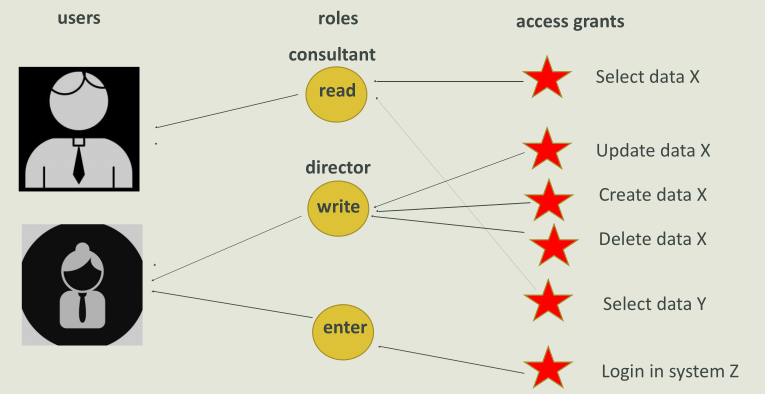
\includegraphics[scale=0.5]{02P/RBAC.png}
    \caption{RBAC.}
    \label{fig:rbac}

  \end{figure}


